\documentclass[aspectratio=169,11pt]{beamer}

\usepackage[T1]{fontenc}
\usepackage[sfdefault]{sourcesanspro}
\usepackage{sfmath}
\usepackage{amsmath,amssymb}
\usepackage{booktabs,tabularx,array,colortbl}
\usepackage{pgfplots}
\usepackage{microtype}
\usepackage{xurl}

\pgfplotsset{compat=1.18}

% -----------------------------------------------------------------------------
% Visual system (colours as in the 8 September deck; type scaled to fit
% the 16:9 frame -- the earlier deck overflowed several frames)
% -----------------------------------------------------------------------------
\definecolor{Navy}{HTML}{18324B}
\definecolor{Teal}{HTML}{138A8A}
\definecolor{Orange}{HTML}{E07A45}
\definecolor{Gold}{HTML}{CAA032}
\definecolor{WarmWhite}{HTML}{F7F4EE}
\definecolor{PaleTeal}{HTML}{E4F0EF}
\definecolor{PaleOrange}{HTML}{F8E9E0}
\definecolor{MidGray}{HTML}{65717C}
\definecolor{LightGray}{HTML}{D8DEE3}

\setbeamertemplate{navigation symbols}{}
\setbeamertemplate{itemize item}{\color{Teal}\raise0.15ex\hbox{\rule{0.55ex}{0.55ex}}}
\setbeamersize{text margin left=9mm,text margin right=9mm}

\setbeamercolor{normal text}{fg=Navy,bg=WarmWhite}
\setbeamercolor{frametitle}{fg=Navy,bg=WarmWhite}
\setbeamercolor{footline}{fg=MidGray,bg=WarmWhite}
\setbeamercolor{structure}{fg=Teal}
\setbeamerfont{normal text}{size=\fontsize{10.5}{12.8}\selectfont}
\setbeamerfont{frametitle}{size=\fontsize{18}{21}\selectfont,series=\bfseries}
\setbeamerfont{footline}{size=\fontsize{6.8}{8}\selectfont}

\setbeamertemplate{frametitle}{%
  \vspace{1.8mm}%
  \insertframetitle\par
  \vspace{0.8mm}%
  {\color{Teal}\rule{19mm}{1.3pt}}%
}

\setbeamertemplate{footline}{%
  \leavevmode%
  \hbox{%
    \begin{beamercolorbox}[wd=.82\paperwidth,ht=2.6ex,dp=1.1ex,leftskip=9mm]{footline}%
      Block-adaptive Bayesian local projections \hspace{0.9em} Current state: 12 September 2026
    \end{beamercolorbox}%
    \begin{beamercolorbox}[wd=.18\paperwidth,ht=2.6ex,dp=1.1ex,rightskip=9mm plus 1fil]{footline}%
      \insertframenumber\,/\,\inserttotalframenumber
    \end{beamercolorbox}%
  }%
}

\newcommand{\keypoint}[1]{\textcolor{Teal}{\textbf{#1}}}
\newcommand{\warning}[1]{\textcolor{Orange}{\textbf{#1}}}
\newcommand{\smallsource}[1]{%
  \par\vfill{\fontsize{7}{8.4}\selectfont\color{MidGray}#1}%
}
\newcommand{\statusrow}[3]{%
  \textcolor{#1}{\bfseries #2} & #3\\[1.2mm]
}
\newcommand{\bigbox}[2]{%
  \colorbox{#1}{\parbox{0.955\textwidth}{\vspace{1.4mm}#2\vspace{1.4mm}}}}

\begin{document}

% -----------------------------------------------------------------------------
% 1. Cover
% -----------------------------------------------------------------------------
{
\setbeamercolor{background canvas}{bg=Navy}
\begin{frame}[plain]
  \color{WarmWhite}
  \vspace{6mm}
  {\color{Teal}\rule{22mm}{2.4pt}}\par
  \vspace{5mm}
  {\fontsize{30}{34}\selectfont\bfseries
    Where does the VAR prior fail?\par}
  \vspace{3mm}
  {\fontsize{18}{22}\selectfont
    Block-adaptive Bayesian local projections\par
    under sparse dynamic misspecification}
  \vfill
  {\fontsize{12.5}{15.5}\selectfont\color{LightGray}
    MSc thesis project \quad Stefano Graziosi \quad 12 September 2026}
  \vspace{2.5mm}
  {\fontsize{10}{12.5}\selectfont\color{LightGray}
    Status: methodological prototype, $R=500$ Monte Carlo evidence, and a first pass at the euro-area application.}
  \vspace{4mm}
\end{frame}
}

% -----------------------------------------------------------------------------
% 2. Motivation
% -----------------------------------------------------------------------------
\begin{frame}{The research question}
  \begin{columns}[T,onlytextwidth]
    \column{0.47\textwidth}
      {\fontsize{13}{15.5}\selectfont\color{Teal}\bfseries Local projections}\par
      \vspace{1.5mm}
      Estimate each horizon directly. They tolerate richer dynamics, but
      impulse responses can be imprecise in modest samples.
    \column{0.06\textwidth}
      \centering\vspace{6mm}{\color{LightGray}\rule{0.7pt}{20mm}}
    \column{0.47\textwidth}
      {\fontsize{13}{15.5}\selectfont\color{Orange}\bfseries VARs}\par
      \vspace{1.5mm}
      Impose one dynamic system across horizons. They gain precision when
      that system is adequate, but transmit misspecification everywhere.
  \end{columns}
  \vspace{4mm}
  {\color{MidGray}
    A global Bayesian LP compromises by shrinking every coefficient block
    toward a VAR-implied centre with the same horizon-specific tightness
    $\lambda_h$.}
  \vspace{4mm}
  \bigbox{PaleTeal}{\fontsize{13.5}{16.5}\selectfont\bfseries
    When the VAR is wrong in one part of the system, can only that part
    of the LP escape the prior, and does it help?}
\end{frame}

% -----------------------------------------------------------------------------
% 3. Method
% -----------------------------------------------------------------------------
\begin{frame}{Block-adaptive VAR-centred shrinkage}
  \vspace{-3mm}
  {\fontsize{11}{13.5}\selectfont
  \begin{align*}
    y_{i,t+h} &= z_t'\beta_{i,h}+u_{i,t+h},\\[-1mm]
    \beta_{i,g,h}-\mu^{\mathrm{BVAR}}_{i,g,h}
      &\sim \mathcal N\!\left(0,\ \sigma^2_{i,h}\lambda_h^2\tau_{i,g,h}^2D_{g,h}\right),
      \qquad \tau_{i,g,h}\sim\mathcal C^+(0,1).
  \end{align*}}
  \vspace{-4mm}
  \begin{columns}[T,onlytextwidth]
    \column{0.62\textwidth}
      In each response equation and horizon, block $g$ collects the $p$
      coefficients on the lags of predictor $g$. Three estimators differ
      only in how $\tau$ is treated:\par
      \vspace{1.5mm}
      \begin{tabular}{@{}ll@{}}
        \keypoint{BLP-FMAR} & $\tau\equiv1$: the published global baseline\\
        \keypoint{BLP-block} & $\tau_{i,g,h}$ independent at every horizon\\
        \keypoint{BLP-pooled} & random walk on $\log\tau_{i,g,h}$ across $h$\\
      \end{tabular}\par
      \vspace{1mm}
      Shrinkage acts on deviations from the BVAR centre, not toward zero.
    \column{0.33\textwidth}
      \keypoint{$\tau_{i,g,h}<1$}\; tighter than the global prior\par
      \vspace{1mm}
      \textbf{$\tau_{i,g,h}=1$}\; the global FMAR baseline\par
      \vspace{1mm}
      \warning{$\tau_{i,g,h}>1$}\; local escape from the VAR
  \end{columns}
  \smallsource{With every $\tau=1$ both adaptive estimators reproduce the FMAR closed form to $3\times10^{-16}$ (912 cells). Baseline: Ferreira, Miranda-Agrippino, Ricco (2025); sampler: Makalic and Schmidt (2016).}
\end{frame}

% -----------------------------------------------------------------------------
% 4. Simulation design
% -----------------------------------------------------------------------------
\begin{frame}{A deliberately diagnostic Monte Carlo design}
  \vspace{-1mm}
  {\fontsize{9}{10.6}\selectfont
  \renewcommand{\arraystretch}{1.0}
  \begin{tabularx}{\textwidth}{>{\bfseries}p{0.13\textwidth} p{0.38\textwidth} X}
    \toprule
    Regime & True dynamics & What the design tests \\
    \midrule
    Correct & Stable VAR(2) & Does unnecessary local flexibility cost precision? \\
    \rowcolor{PaleTeal}
    Sparse & VAR(3), only $A_3(3,1)=-0.30$ missing from the fitted VAR(2) & Does block 1 escape in the $y_3$ equation, where the transmission prior is wrong? \\
    Intermediate & VAR(3), nonzero first \emph{column} of $A_3$ & The same block wrong in \emph{every} equation \\
    Dense & VARMA(2,1), dense MA matrix & Does the advantage vanish when no block is responsible? \\
    \bottomrule
  \end{tabularx}}
  \vspace{1.5mm}
  {\fontsize{9.4}{11.2}\selectfont
  \keypoint{Headline experiment.} $K=3$, $T=200$, fitted $p=2$, $H=20$; $R=500$ (correct, sparse), $R=250$ (intermediate, dense); a recursive unit shock to $y_1$.
  \keypoint{Comparison.} LP, BVAR, BLP-FMAR, BLP-block, BLP-pooled on the same samples; paired Monte Carlo $t$ statistics; integrated RMSE over $h\geq2$; $\tau$ localisation against a measured null.}
\end{frame}

% -----------------------------------------------------------------------------
% 5. Current implementation state
% -----------------------------------------------------------------------------
\begin{frame}{What is implemented now}
  \vspace{-1.5mm}
  {\fontsize{9.5}{11.4}\selectfont
  \renewcommand{\arraystretch}{1.0}
  \begin{tabularx}{\textwidth}{p{0.18\textwidth} X}
    \statusrow{Teal}{Method}{FMAR BVAR and global BLP; block-adaptive Gibbs sampler; horizon-pooled sampler (checkerboard Metropolis on $\log\tau$); HAC bands; Rao--Blackwellised point estimates.}
    \statusrow{Teal}{Fair benchmark}{$h=1$ estimated as an LP for every estimator; integrated RMSE over $h=2..H$; common $\lambda_h$; paired comparisons on identical samples.}
    \statusrow{Teal}{Evidence}{Five-estimator headline runs for all four DGPs, a 13-cell exploratory grid, a sensitivity analysis of the remaining approximations; every table regenerated from stored files.}
    % (kept to two lines)
    \statusrow{Teal}{Verification}{17 assertion tests pass in MATLAB R2025b (12 minutes): exact nesting, chunk-exact parallel runs, the prior-scale floor, the held-block option, the empirical pipeline.}
    \statusrow{Gold}{Empirical}{Euro-area data assembled and validated; the full pipeline has run (five estimators, dose--response in $p$, JK split, coherence, null at $R=500$); three corrections were needed on the real data.}
  \end{tabularx}}
  \vspace{0.5mm}
  \bigbox{PaleOrange}{\fontsize{9}{11}\selectfont
      \textbf{Caveats.} The fidelity test against the original FMAR code still skips (package not installed); the raw outcome series are third-party data, not in the repository.}
\end{frame}

% -----------------------------------------------------------------------------
% 6. Evidence
% Values from results/mc_headline_sparse.mat, s.tau_stats.{block,pooled}.tau_bar(3,:,:)
% -----------------------------------------------------------------------------
\begin{frame}{The scales locate the failure; pooling makes them sharp}
  \vspace{-4mm}
  \begin{columns}[T,onlytextwidth]
    \column{0.57\textwidth}
      \begin{tikzpicture}
      \begin{axis}[
        name=ind,
        width=0.52\linewidth, height=0.43\textheight,
        xmin=1,xmax=20, ymin=0.2,ymax=2.4,
        xtick={1,5,10,15,20}, ytick={0.5,1,1.5,2},
        xlabel={Horizon $h$}, ylabel={Average posterior $\tau_{3,g,h}$},
        title={\fontsize{8.5}{10}\selectfont independent $\tau$},
        label style={font=\fontsize{8.5}{10}\selectfont,color=Navy},
        tick label style={font=\fontsize{7.5}{9}\selectfont,color=Navy},
        title style={color=Navy},
        axis line style={color=MidGray}, grid=major,
        grid style={color=LightGray,line width=0.35pt}
      ]
      \addplot+[color=Teal,line width=2pt,mark=none] coordinates {
        (1,0.5643) (2,2.1713) (3,1.5197) (4,1.5903) (5,1.6019) (6,1.5102) (7,1.4066) (8,1.3191) (9,1.2126) (10,1.1760) (11,1.1254) (12,1.1241) (13,1.1226) (14,1.1301) (15,1.1386) (16,1.1610) (17,1.1734) (18,1.1783) (19,1.2228) (20,1.2311)};
      \addplot+[color=Orange,line width=1.4pt,mark=none] coordinates {
        (1,0.5586) (2,0.6033) (3,0.7363) (4,0.7815) (5,0.8216) (6,0.8870) (7,0.9501) (8,0.9943) (9,1.0234) (10,1.0536) (11,1.0644) (12,1.0689) (13,1.0802) (14,1.0781) (15,1.0919) (16,1.0860) (17,1.1065) (18,1.0976) (19,1.1165) (20,1.1114)};
      \addplot+[color=Gold,line width=1.4pt,mark=none] coordinates {
        (1,0.5705) (2,0.5306) (3,0.6489) (4,0.7137) (5,0.7603) (6,0.8089) (7,0.8546) (8,0.9066) (9,0.9460) (10,0.9831) (11,1.0051) (12,1.0268) (13,1.0383) (14,1.0680) (15,1.0731) (16,1.0727) (17,1.0672) (18,1.0723) (19,1.0609) (20,1.0701)};
      \addplot+[color=Navy,dashed,line width=0.8pt,mark=none] coordinates {(1,1) (20,1)};
      \end{axis}
      \begin{axis}[
        at={(ind.east)}, anchor=west, xshift=8mm,
        width=0.52\linewidth, height=0.43\textheight,
        xmin=1,xmax=20, ymin=0.2,ymax=2.4,
        xtick={1,5,10,15,20}, ytick={0.5,1,1.5,2}, yticklabels={},
        xlabel={Horizon $h$},
        title={\fontsize{8.5}{10}\selectfont pooled across $h$},
        label style={font=\fontsize{8.5}{10}\selectfont,color=Navy},
        tick label style={font=\fontsize{7.5}{9}\selectfont,color=Navy},
        title style={color=Navy},
        axis line style={color=MidGray}, grid=major,
        grid style={color=LightGray,line width=0.35pt},
        legend style={at={(0.97,0.97)},anchor=north east,draw=none,fill=WarmWhite,
                      font=\fontsize{7}{8.5}\selectfont,row sep=-1pt}
      ]
      \addplot+[color=Teal,line width=2pt,mark=none] coordinates {
        (1,1.2030) (2,1.2986) (3,1.2860) (4,1.2812) (5,1.2649) (6,1.2304) (7,1.1823) (8,1.1295) (9,1.0761) (10,1.0300) (11,0.9921) (12,0.9636) (13,0.9443) (14,0.9327) (15,0.9289) (16,0.9306) (17,0.9378) (18,0.9506) (19,0.9683) (20,0.9908)};
      \addlegendentry{block 1, lags of $y_1$}
      \addplot+[color=Orange,line width=1.4pt,mark=none] coordinates {
        (1,0.3963) (2,0.3876) (3,0.3942) (4,0.4075) (5,0.4267) (6,0.4510) (7,0.4785) (8,0.5033) (9,0.5246) (10,0.5420) (11,0.5551) (12,0.5648) (13,0.5739) (14,0.5811) (15,0.5891) (16,0.5966) (17,0.6078) (18,0.6198) (19,0.6333) (20,0.6502)};
      \addlegendentry{block 2, lags of $y_2$}
      \addplot+[color=Gold,line width=1.4pt,mark=none] coordinates {
        (1,0.3531) (2,0.3409) (3,0.3438) (4,0.3553) (5,0.3720) (6,0.3930) (7,0.4172) (8,0.4432) (9,0.4687) (10,0.4930) (11,0.5156) (12,0.5356) (13,0.5546) (14,0.5694) (15,0.5810) (16,0.5900) (17,0.5976) (18,0.6063) (19,0.6156) (20,0.6296)};
      \addlegendentry{block 3, lags of $y_3$}
      \addplot+[color=Navy,dashed,line width=0.8pt,mark=none] coordinates {(1,1) (20,1)};
      \end{axis}
      \end{tikzpicture}
      {\fontsize{7.8}{9.2}\selectfont\color{MidGray}
       Sparse DGP, $y_3$ equation, 500 replications.}
    \column{0.41\textwidth}
      {\fontsize{10.3}{12.5}\selectfont
      \keypoint{Localisation, early horizons.} The true (equation, block) cell ranks first in \textbf{97\%} of replications; \textbf{37\%} on the correct DGP.\par
      \vspace{1mm}
      \keypoint{Detection.} Some cell has $P(\tau>1)>0.5$ in \textbf{74\%} of sparse replications, \textbf{3\%} of correct ones.\par
      \vspace{2mm}
      {\fontsize{9.5}{11.4}\selectfont
      \renewcommand{\arraystretch}{1.05}
      \begin{tabular}{@{}llccc@{}}
        \toprule
        & & early & all $h\!\geq\!2$ & late \\
        \midrule
        sparse  & block  & .968 & 1.012 & 1.040 \\
                & pooled & .973 & \textbf{1.003} & 1.021 \\
        correct & block  & .965 & 1.011 & 1.031 \\
                & pooled & .949 & \textbf{.988} & 1.005 \\
        \bottomrule
      \end{tabular}}\par
      \vspace{0.5mm}
      {\fontsize{8.2}{9.8}\selectfont\color{MidGray}Paired RMSE ratio vs BLP-FMAR, $<1$ = adaptation helps; $|t|>3$ except the bold entries.}}
  \end{columns}
\end{frame}

% -----------------------------------------------------------------------------
% 7. Claim boundary
% -----------------------------------------------------------------------------
\begin{frame}{What the project can claim today}
  \vspace{-1mm}
  {\fontsize{9.6}{11.6}\selectfont
  \renewcommand{\arraystretch}{1.0}
  \begin{tabularx}{\textwidth}{p{0.2\textwidth} X}
    \statusrow{Teal}{Established}{A calibrated, localised diagnostic of prior--data conflict: the true cell is found 97\% of the time against a 37\% measured null; an honest \emph{no} on the dense DGP; monotone in conflict strength; exactly nested in FMAR.}
    \statusrow{Teal}{Established}{Adaptation lowers RMSE early and raises it late on every DGP but one; pooling keeps the early gain and halves the late penalty, so the adaptive layer is RMSE-neutral.}
    \statusrow{Gold}{Finding}{Knowing \emph{where} a VAR prior fails does not imply that escaping there helps: on the intermediate DGP the map localises perfectly and adaptation is worse at every horizon.}
    \statusrow{Orange}{Not established}{Integrated-RMSE superiority; a $\tau$ threshold that transfers across specifications (the null moved from 0.42 to 0.68 with the fitted lag order); any statement about euro-area transmission.}
  \end{tabularx}}
  \vspace{0.5mm}
  \bigbox{PaleTeal}{\fontsize{10.5}{12.8}\selectfont\bfseries
      Framing the evidence supports: a specification diagnostic for VAR-centred local projections, with horizon pooling as the refinement that makes it sharp and RMSE-neutral.}
\end{frame}

% -----------------------------------------------------------------------------
% 8. Euro-area application: what the data forced
% -----------------------------------------------------------------------------
\begin{frame}{Euro area: three things the real data forced}
  \vspace{-1mm}
  {\fontsize{9.8}{11.9}\selectfont
  Monthly 2000--2019, $K=5$: EA-EMPD 1-year OIS surprise (internal instrument, ordered first), 12-month Euribor, industrial production, HICP, EURO STOXX 50; $p=12$, $H=48$.
  \vspace{1mm}
  \renewcommand{\arraystretch}{1.0}
  \begin{tabularx}{\textwidth}{p{0.2\textwidth} X}
    \statusrow{Orange}{Weak instrument}{The surprise innovation moves the rate innovation with $t=0.77$ ($F=0.6$), not the $F\approx4$ budgeted: a monthly-\emph{average} indicator smears events over two months, and the largest surprises sit in late 2008 against 90\,bp rate falls. The $\tau$ diagnostic does not depend on this; the IRFs and the 25\,bp scale do.}
    \statusrow{Orange}{Prior scale}{FMAR's Newey--West scale falls to a fifth of the variance for the near-white-noise surprise; the marginal likelihood answers by driving the \emph{global} $\lambda_h$ to 0.01, bimodal at 28 of 48 horizons. A floor at the residual variance (inert on the simulations) restores a smooth path.}
    \statusrow{Orange}{Instrument block}{One large contemporaneous coefficient and eleven near-zero lags violate the block prior's common scale; freed, the block collapsed and pulled the identifying coefficient to the VAR centre. It is held at $\tau=1$; the diagnostic is read on the four level blocks.}
  \end{tabularx}}
  \smallsource{Each choice defaults to the published behaviour, is pinned by a test and documented in \texttt{empirical/README\_EMPIRICAL.md}.}
\end{frame}

% -----------------------------------------------------------------------------
% 9. Euro-area application: what the map says
% -----------------------------------------------------------------------------
\begin{frame}{Euro area: the $\tau$ map and its null}
  \vspace{-2mm}
  \begin{columns}[T,onlytextwidth]
    \column{0.54\textwidth}
      {\fontsize{9.4}{11.2}\selectfont
      Early-horizon mean scale $\bar\tau_{i,g}$, $h=2..12$, pooled (independent in brackets); rows = equations, columns = level blocks.\par
      \vspace{1mm}
      {\fontsize{9.4}{11.2}\selectfont
      \renewcommand{\arraystretch}{1.05}
      \begin{tabular}{@{}lcccc@{}}
        \toprule
        & i1y & ip & hicp & stoxx \\
        \midrule
        mps   & 0.07 (0.5) & 0.10 (0.6) & 0.05 (0.6) & 0.09 (0.7) \\
        i1y   & 4.6 (2.0) & 2.4 (1.3) & 0.9 (0.9) & 2.7 (1.7) \\
        ip    & \textbf{7.6} (5.3) & 4.4 (3.2) & 2.1 (1.9) & 1.8 (1.3) \\
        hicp  & 3.3 (2.4) & 2.3 (1.8) & \textbf{10.0} (9.4) & 3.0 (2.3) \\
        stoxx & 4.4 (2.6) & 3.3 (1.9) & 0.4 (0.6) & 0.3 (0.7) \\
        \bottomrule
      \end{tabular}}\par
      \vspace{1mm}
      \keypoint{Negative control passes} (surprise equation quiet at every $p$); \keypoint{coherence holds} (blocks with $\tau>2$ closer to their unshrunk value than under FMAR in 100\% of cells).}
    \column{0.43\textwidth}
      {\fontsize{9.4}{11.2}\selectfont
      \keypoint{Against the simulated null} ($R=500$ datasets from the fitted BVAR through the whole pipeline):\par
      \vspace{0.8mm}
      Equation-wide q95 of the largest $\bar\tau$ is \textbf{5.5--8.5}: the null is wide. Two cells survive: the \textbf{HICP own block} (9.4 vs 7.0; pooled 10.0 vs 8.3) and the \textbf{rate block in the IP equation} (pooled 7.6 vs 7.4). All rate-block cells in the i1y and stoxx equations are inside their null.\par
      \vspace{1mm}
      \warning{Through the protocol} the dose--response in $p$ is flat (1 / 1 / 2 escapes at $p=2/6/12$), and in the level system without the surprise only the HICP block survives its own null.}
  \end{columns}
  \smallsource{Sources: \texttt{results/tau\_protocol\_p12.csv} and \texttt{empirical/docs/CH7\_RESULTS.md}.}
\end{frame}

% -----------------------------------------------------------------------------
% 10. Roadmap
% -----------------------------------------------------------------------------
\begin{frame}{Highest-return next steps}
  \vspace{-1mm}
  {\fontsize{10.2}{12.4}\selectfont
  \begin{tabularx}{\textwidth}{>{\color{Teal}\bfseries\fontsize{18}{21}\selectfont}p{0.05\textwidth} X}
    1 & \textbf{Treat the instrument the AGKL way.} Zero restrictions on the surprise block remove the drag on $\lambda_h$ at the source instead of rescaling it; joint selection of $\lambda_h$ and the block scales is the general version.\\[2mm]
    2 & \textbf{A stronger policy indicator.} An end-of-month 1-year OIS level instead of the monthly-average Euribor removes the two-month smearing and the 2008--2012 credit premium.\\[2mm]
    3 & \textbf{Robustness the design lists.} The 3-month surprise, the speeches-augmented series (all months covered), the $K=7$ system with loans and spreads.\\[2mm]
    4 & \textbf{Method.} A non-centred parameterisation for the pooled $\log\tau$ chain (ESS 10--70 of 700); a factorial grid to see interactions between sparsity and sample size.\\
  \end{tabularx}}
  \vfill
  \bigbox{PaleTeal}{\fontsize{11}{13.5}\selectfont\bfseries
      Best use of supervision: agree the diagnostic framing and the instrument treatment before writing the empirical chapter.}
\end{frame}

% -----------------------------------------------------------------------------
% 11. Restart map
% -----------------------------------------------------------------------------
\begin{frame}{Restart map}
  \vspace{-1mm}
  {\fontsize{9.6}{11.6}\selectfont
  \renewcommand{\arraystretch}{1.08}
  \begin{tabularx}{\textwidth}{>{\bfseries\color{Teal}}p{0.2\textwidth} X}
    Reorient & \texttt{docs/PROJECT\_EXPLAINED.md} (the procedure and every file in plain language), then \texttt{docs/RESULTS.md} and \texttt{empirical/docs/CH7\_RESULTS.md}.\\[1.5mm]
    Test & \texttt{cd tests; run\_all\_tests} (12 minutes in MATLAB). Set \texttt{FMAR\_PATH} for the fidelity test against the original package.\\[1.5mm]
    Simulation evidence & \texttt{report\_montecarlo('results/mc\_headline\_sparse.mat')}; \texttt{results/REPORT.txt} has every table.\\[1.5mm]
    Empirical chapter & \texttt{SMOKE\_TEST\_EMPIRICAL}, then \texttt{RUN\_EMPIRICAL} (4 minutes) and \texttt{run\_null\_calibration} (85 minutes at $R=500$); outputs carry the tags \texttt{p12}, \texttt{p12\_nofloor}, \texttt{p12\_allblocks}, \texttt{\_levels}.\\[1.5mm]
    Method work & \texttt{estimate\_blp\_blockpooled.m}, \texttt{gibbs\_block\_pooled\_horizons.m}, \texttt{select\_lambda\_fmar.m}, \texttt{fmar\_prior\_scale.m}.\\
  \end{tabularx}}
  \vfill
  {\fontsize{12.5}{15.5}\selectfont\bfseries
   First question on return: with the instrument block restricted the AGKL way, does the euro-area map keep the HICP and interest-rate blocks as its two features?}
\end{frame}

\end{document}
